
% Introdução
%--------------------------------------
\chapter{Introdução}

O capítulo introdutório deverá ser apresentado neste ficheiro com toda a informação necessária à compreensão do tema/assunto do trabalho \cite{CitekeyMastersthesis}\cite{CitekeyBook}. 

Deverão constar os conceitos fundamentais relacionados com o tema do  trabalho, devendo terminar com a descrição genérica da organização do documento.

No que segue é apresentada a forma de importar o \textit{template} para o programa \textit{Overleaf} e como é constituído o próprio \textit{template}  em \LaTeX~ sugerido aos alunos. Para além disso, também se explica como criar e juntar a capa do trabalho ao documento.

Os ficheiros do \textit{template} estão disponíveis na pasta Template4LaTeX4ISEC que está disponível no \textit{site} do ISEC -> serviços académicos $\rightarrow$ formulários $\rightarrow$ mestrado $\rightarrow$ Template para Teses, Projetos e Relatórios de Estágio $\rightarrow$ ... \\
Dentro desta pasta encontram-se dois ficheiros ZIP relativos a dois projetos. Um dos projetos é o \textit{template} (projeto limpo, apenas com o esqueleto de base) e o outro é um  exemplo que corresponde a um projeto customizado com um nome diferente e com exemplos incluídos. Nessa pasta encontram-se ainda dois ficheiros PDF, em que cada um corresponde à versão impressa de cada um dos projetos supra mencionados.

\section{Como importar o \textit{template} para o Overleaf}
    Nesta secção explicam-se os passos que devem ser seguidos para usar este \textit{template}:
    \begin{enumerate}
        \item Criar conta no Overleaf;
        \item No Overleaf, escolher \textbf{New Project} $\rightarrow$ \textbf{Upload Project} $\rightarrow$ escolher o projeto de nome \textbf{ISEC LaTeX template} previamente guardado em disco tal como ilustra a  Figura~\ref{fig-upload}.
        \item Para fazer o \textit{rename} do projeto, deve selecionar o projeto e proceder como ilustra a Figura~\ref{fig-rename}.% ilustra os passos enunciados anteriormente.
    \end{enumerate}
    
    \begin{figure}[htp]
    	\centering
    	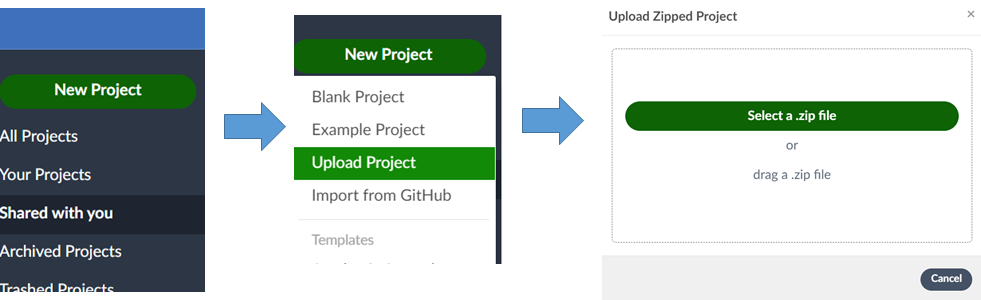
\includegraphics[width=0.8\textwidth]{Figuras/UploadProject}
     \caption{\small{Passos para criar um projeto com base no projeto \textit{template}}}
    	\label{fig-upload}
    \end{figure}

     \begin{figure}[htp]
    	\centering
    	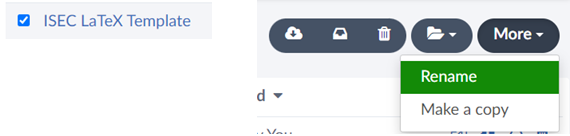
\includegraphics[width=0.6\textwidth]{Figuras/RenameProject}
     \caption{\small{Passos para fazer o \textit{rename} de um projeto}}
    	\label{fig-rename}
    \end{figure}
    
\section{Constituição do \textit{template}}
    
    O \textit{template} é constituído por 5 pastas e 3 ficheiros, cujo teor se descreve de seguida:
    
    \begin{itemize}
        \item Ficheiro \textbf{main.tex}: possui o esqueleto do documento. \textbf{Apenas} deve editar este ficheiro para: 
            \begin{itemize}
                  \item definir o título do trabalho e o nome do autor (procurar por Obs\#2);
                  \item acrescentar ou retirar elementos da estrutura do trabalho como, por exemplo, capítulos ou anexos;
                  \item escolher a formatação das referências bibliográficas: IEEE ou APA (procurar por Obs\#3);
                  \item definir o nome dos anexos (procurar por Obs\#4 e Obs\#5).  
            \end{itemize}
        
        \item Ficheiro \textbf{extras.sty}: na elaboração do documento pode revelar-se necessário a utilização de instruções ou ficheiros adicionais (p. ex., packages, comandos, etc.) devendo os mesmos ser inseridos neste ficheiro; Por exemplo, nas linhas 13, 14 e 15 do ficheiro \verb|extras.sty| estão incluídas as instruções necessárias que ativam as funcionalidades de hipertexto, links e endereços web.
         
        \item Ficheiro \textbf{bibliografia.bib}: é aqui que devem ser colocados os registos de cada uma das referências bibliográficas; neste ficheiro exemplo encontram um  registo de cada um dos possíveis tipos de referências bibliográficas;
        
        \item Pasta \textbf{Setup}: nesta pasta estão incluídos alguns ficheiros específicos do \textit{template}; não pode ser modificada pelo utilizador, sob pena de alterar as características do \textit{template};
    
        \item Pasta \textbf{Início}: todos os ficheiros iniciais do relatório (automaticamente numerados com numeração romana no texto), com extensão *.tex, estão contidos nesta pasta; todos eles devem ser editados com exceção do ficheiro \verb|capa.pdf| e 
        do ficheiro \verb|capa.docx| (ficheiro que apenas se encontra na pasta do projeto gravado localmente no disco). Estes dois ficheiros dizem respeito à criação da capa e são abordados na secção seguinte;
        
        \item Pasta \textbf{Figuras}: é nesta pasta que devem ser colocadas as figuras do documento. Devem ter extensão *.png. Para carregar uma figura para dentro desta pasta devem fazer \textit{Upload} (comando seta no lado esquerdo superior) $\rightarrow$ arrastar a figura para dentro da caixa destino;
    
        \item Pasta \textbf{Capítulos}: dentro desta pasta é onde devem ser colocados os ficheiros *.tex relativos a cada capítulo. Considera-se que o primeiro capítulo é a introdução do trabalho e que o último capítulo é a conclusão do trabalho. Para criar um novo ficheiro *.tex deverá escolher o comando \textit{New File} (comando no lado esquerdo superior);
    
        \item Pasta \textbf{Anexos}: é nesta pasta que devem estar localizados os anexos. Para criar o ficheiro *.tex para um novo anexo, deve proceder de forma idêntica à criação de um novo capítulo.
        
    \end{itemize}
    
    Pode criar novas pastas com o comando \textit{New Folder} (comando no lado esquerdo superior).

\section{Criação da capa do trabalho}

    Para criar a capa do trabalho, deve extrair o conteúdo do ficheiro ZIP associado ao \textit{template}. Deve procurar o ficheiro 
    \verb|capa.docx|, que está dentro da pasta \textbf{Inicio} e customizá-lo. Depois, deve gerar o correspondente ficheiro em formato PDF \verb|capa.pdf| e efetuar o \textit{Upload} desse ficheiro para dentro da pasta \textbf{Inicio} do projeto no Overleaf.
    
\section{Estrutura do documento}
    No Capítulo \ref{cap2} são apresentados alguns exemplos de escrita em \LaTeX, onde são, por exemplo, apresentadas fórmulas matemáticas, tabelas, imagens e muito mais.
    
    No tocante às referências bibliográficas e à escolha do respetivo estilo, deve ser consultado o Capítulo \ref{cap3}.
    
    O trabalho termina com o Capítulo \ref{conclusao} onde são apresentadas as conclusões.